\chapter{Introduction}
\label{chap:introduction}

\section{Background and Motivation}
\label{sec:intro_background}

In the contemporary healthcare landscape, clinical data is generated across an increasingly heterogeneous array of institutional and private touchpoints, ranging from tertiary hospital electronic health record (EHR) installations to standalone outpatient clinics, diagnostic pathology laboratories, and ambulatory pharmacies. In emerging economies such as India, this heterogeneity is exacerbated by the absence of a universally enforced, unified digital health infrastructure. While initiatives such as the Ayushman Bharat Digital Mission (ABDM)~\cite{nha2022abdm} have introduced foundational architectural standards, the vast majority of patient health records continue to exist as unlinked, non-standardized artifacts. These encompass physical paper prescriptions, scanned photographic receipts, non-searchable portable document formats (PDFs), and proprietary hospital discharge summaries stored across siloed databases~\cite{jensen2012mining}. 

Consequently, a patient undergoing treatment across multiple clinical facilities over a five-to-ten-year horizon inevitably accumulates an episodic, fragmented medical history. When presenting to a clinician during an acute exacerbation or routine consultation, the clinician is confronted with an overwhelming cognitive burden: they must rapidly digest dozens of historical documents, manually cross-reference numerical laboratory values across conflicting reference intervals, and reconstruct medication timelines within strict consultation time constraints (often fewer than five to eight minutes per patient).

The rapid advent of Generative Artificial Intelligence and Large Language Models (LLMs) has prompted significant interest in deploying conversational AI agents to automate clinical summarization and patient-facing inquiry~\cite{wornow2023shaky,yang2022gatortron}. However, commercial foundation models operating in zero-shot or generic prompt-based settings present profound failure modes in clinical domains:
\begin{enumerate}
    \item \textbf{Stochastic Hallucination and Unauditable Assertions}: Generative language models predict plausible continuation tokens based on probabilistic distribution matching rather than deterministic clinical evidence. When queried regarding a patient's historical laboratory trends, an ungrounded model may invent normal ranges, hallucinate negative findings, or cite non-existent clinical trials, posing catastrophic risks to patient safety~\cite{pampari2018emrqa}.
    \item \textbf{Numerical and Temporal Blindness}: Dense vector representations alone (standard semantic embedding search) frequently fail to distinguish between critical temporal nuances (e.g., distinguishing between a Fasting Blood Glucose of $146\text{ mg/dL}$ recorded in 2021 versus $98\text{ mg/dL}$ recorded in 2026) and struggle with unit discrepancies (e.g., converting $\text{mmol/L}$ to $\text{mg/dL}$)~\cite{gao2023rag_survey}.
    \item \textbf{Sovereignty and Privacy Vulnerabilities}: Proprietary cloud-hosted clinical AI solutions require transmitting unencrypted protected health information (PHI) across public internet boundaries to external cloud endpoints, violating emerging data protection mandates such as India's Digital Personal Data Protection (DPDP) Act 2023 and the Health Insurance Portability and Accountability Act (HIPAA)~\cite{nha2022abdm}.
    \item \textbf{Linguistic Marginalization in Low-Resource Indic Vernaculars}: The majority of conversational clinical AI platforms are optimized strictly for standard English or high-resource Romance languages. In multilingual nations, linguistic barriers prevent patients from effectively interrogating their own medical histories in their native mother tongue (e.g., Odia, Bengali, Hindi, Telugu, Tamil).
\end{enumerate}

To resolve these pressing healthcare challenges, this project conceives, engineers, and validates \textbf{ChronaNexus}: an AI-powered longitudinal medical intelligence and auditable clinical decision-support platform designed to transform fragmented, episodic health records into a deterministic, chronologically ordered, and mathematically audited knowledge graph.


\section{Problem Statement}
\label{sec:intro_problem}

Contemporary electronic health record workflows lack an auditable, privacy-first mechanism to synthesize multi-year, multi-facility medical histories into deterministic clinical insights. When clinicians and patients interrogate longitudinal health records using conversational artificial intelligence, conventional Retrieval-Augmented Generation (RAG) pipelines exhibit critical limitations:
\begin{itemize}
    \item \textbf{Claim-Context Disconnect}: Generated clinical answers frequently contain assertions that are neither entailed nor supported by the underlying source documents, yet are delivered with high linguistic confidence.
    \item \textbf{Unchecked Benchmark Leakage}: Contemporary clinical claim verification evaluations often suffer from synthetic test set leakage, wherein surface lexical cues allow naive heuristics to appear performant while failing on complex clinical entailment.
    \item \textbf{Absence of Local-First Execution}: Dependency on proprietary third-party cloud APIs jeopardizes patient data sovereignty and imposes recurring operational latency and cost overheads that preclude deployment in resource-constrained community clinics.
\end{itemize}

Formally, the research and engineering problem addressed by ChronaNexus is defined as follows:
\begin{quote}
\textit{How can an asynchronous, privacy-preserving clinical intelligence platform ingest heterogeneous multi-year patient records, construct an accurate chronological clinical timeline, retrieve evidence via dual-channel semantic and lexical fusion, verify all generated clinical assertions through an asymmetric hybrid symbolic-neural framework with guaranteed auditability, and provide low-latency multilingual voice consultations across Indic languages?}
\end{quote}


\section{Project Objectives}
\label{sec:intro_objectives}

To address the defined problem systematically, the ChronaNexus project is partitioned into seven distinct, measurable objectives. Table~\ref{tab:1_1_objectives} outlines these objectives alongside their corresponding engineering modules, architectural tiers, and verification metrics.

\small
\begin{longtable}{@{}p{0.12\linewidth} p{0.31\linewidth} p{0.24\linewidth} p{0.25\linewidth}@{}}
\caption{Project objectives, corresponding system modules, and verification criteria}\label{tab:1_1_objectives} \\
\toprule
\textbf{Objective} & \textbf{Core Goal} & \textbf{Module / Tier} & \textbf{Verification Metric} \\
\midrule
\endfirsthead
\toprule
\multicolumn{4}{c}{\small\textit{Project objectives, modules, and verification criteria (Continued)}} \\[4pt]
\midrule
\textbf{Objective} & \textbf{Core Goal} & \textbf{Module / Tier} & \textbf{Verification Metric} \\
\midrule
\endhead
\midrule
\multicolumn{4}{r}{\footnotesize\textit{Continued on next page...}} \\
\bottomrule
\endfoot
\bottomrule
\endlastfoot
\textbf{OBJ-1} & Ingest, extract, and deduplicate multi-format medical PDFs and clinical images. & Document Vault (\texttt{PyMuPDF} + SHA-256 Engine) & $100\%$ byte-level deduplication; error-free table extraction. \\
\textbf{OBJ-2} & Standardize clinical entities using canonical ontologies (LOINC, RxNorm, ICD-10). & Clinical Terminology Normalizer & Mapping $>95\%$ of target clinical analytes and medications. \\
\textbf{OBJ-3} & Synthesize longitudinal timeline with deterministic delta trend computation. & Timeline \& Structured Query Engine & Zero-drift chronological ordering (2019--2026); exact delta matching. \\
\textbf{OBJ-4} & Implement dual-channel hybrid retrieval combining dense vectors and lexical search. & Hybrid RAG Engine (\texttt{ChromaDB} + BM25 Okapi) & Reciprocal Rank Fusion ($k=60$) outperforming single-channel retrieval. \\
\textbf{OBJ-5} & Construct an asymmetric hybrid evidence verification pipeline with audit logging. & Evidence Grounding \& Claim Verifier & $86.00\%$ overall verification accuracy; $100\%$ citation attribution precision. \\
\textbf{OBJ-6} & Provide multilingual voice interaction across six languages with regional synthesis. & Indic Phonetic Bridge \& Neural Speech Streamer & $<1.5\text{ s}$ voice response latency; authentic native cadence for Indic speech. \\
\textbf{OBJ-7} & Implement emergency SOS triage dispatch with nearest medical facility discovery. & 108 Emergency Dispatch \& Geolocation Engine & Automatic dispatch payload generation with Haversine distance ranking. \\
\end{longtable}
\normalsize


\section{Scope of the Project}
\label{sec:intro_scope}

To ensure clinical safety, architectural rigor, and engineering feasibility, the operational boundaries of the ChronaNexus platform are formally demarcated:

\subsection{In-Scope System Capabilities}
\begin{itemize}
    \item \textbf{Multi-Format Ingestion}: Parsing and extracting tabular laboratory data, clinical notes, and medication regimens from native and scanned medical PDFs.
    \item \textbf{Longitudinal Synthesis}: Normalizing heterogeneous temporal records into a unified chronological patient timeline spanning multi-year intervals (validated on synthetic datasets covering 2019 to 2026).
    \item \textbf{Dual-Channel Hybrid Retrieval}: Fusing dense vector similarity (\texttt{BAAI/\allowbreak bge-small-\allowbreak en-v1.5}) with lexical keyword matching (BM25 Okapi) via Reciprocal Rank Fusion ($k=60$).
    \item \textbf{Deterministic Evidence Verification}: Enforcing a two-tier verification cascade comprising deterministic symbolic regex rules (Tier 1) and neural Natural Language Inference (Tier 2) to audit generated claims against retrieved context.
    \item \textbf{Auditable Citation Badging}: Emitting verifiable, clickable citation references linked directly to the underlying source document ID, page number, and text chunk.
    \item \textbf{Multilingual Voice Synthesis}: Enabling clinical voice consultation across six languages (English, Hindi, Odia, Telugu, Tamil, Bengali) via a dedicated Unicode phonetic bridge.
    \item \textbf{Emergency Triage Dispatch}: Structuring real-time emergency clinical payloads (blood group, critical allergies, recent vitals) alongside OpenStreetMap Overpass API hospital discovery.
\end{itemize}

\subsection{Architectural Scaffolding and Simulation Elements}
\begin{itemize}
    \item \textbf{Emergency 108 Telephony Integration}: The physical GSM/PSTN call placement and SMS gateway integration to municipal emergency services are implemented as validated architectural mock adapters rather than live carrier trunks, ensuring repeatable test execution without overloading civic infrastructure.
    \item \textbf{Synthetic Patient Data Generation}: Clinical evaluation is executed across an ethically constructed, ten-document synthetic longitudinal medical record corpus to ensure zero exposure of private patient data while maintaining clinical fidelity.
\end{itemize}

\subsection{Explicitly Out-of-Scope Capabilities}
\begin{itemize}
    \item \textbf{Autonomous Clinical Diagnosis}: ChronaNexus is strictly an assistive clinical decision-support and record-synthesis platform. It does not replace certified medical professionals, does not prescribe pharmaceutical regimens autonomously, and issues explicit fail-closed disclaimers on ambiguous inputs.
    \item \textbf{Continuous Biometric Sensor Streaming}: Ingestion of real-time telemetry from wearable IoMT hardware (such as continuous glucose monitors) is reserved for future enterprise releases.
\end{itemize}


\section{Proposed Approach}
\label{sec:intro_approach}

The proposed approach of ChronaNexus departs from conventional black-box conversational systems by enforcing an asymmetric, dual-channel reasoning architecture. Figure~\ref{fig:1_1_workflow} illustrates the end-to-end clinical intelligence lifecycle.

\begin{figure}[htbp]
    \centering
    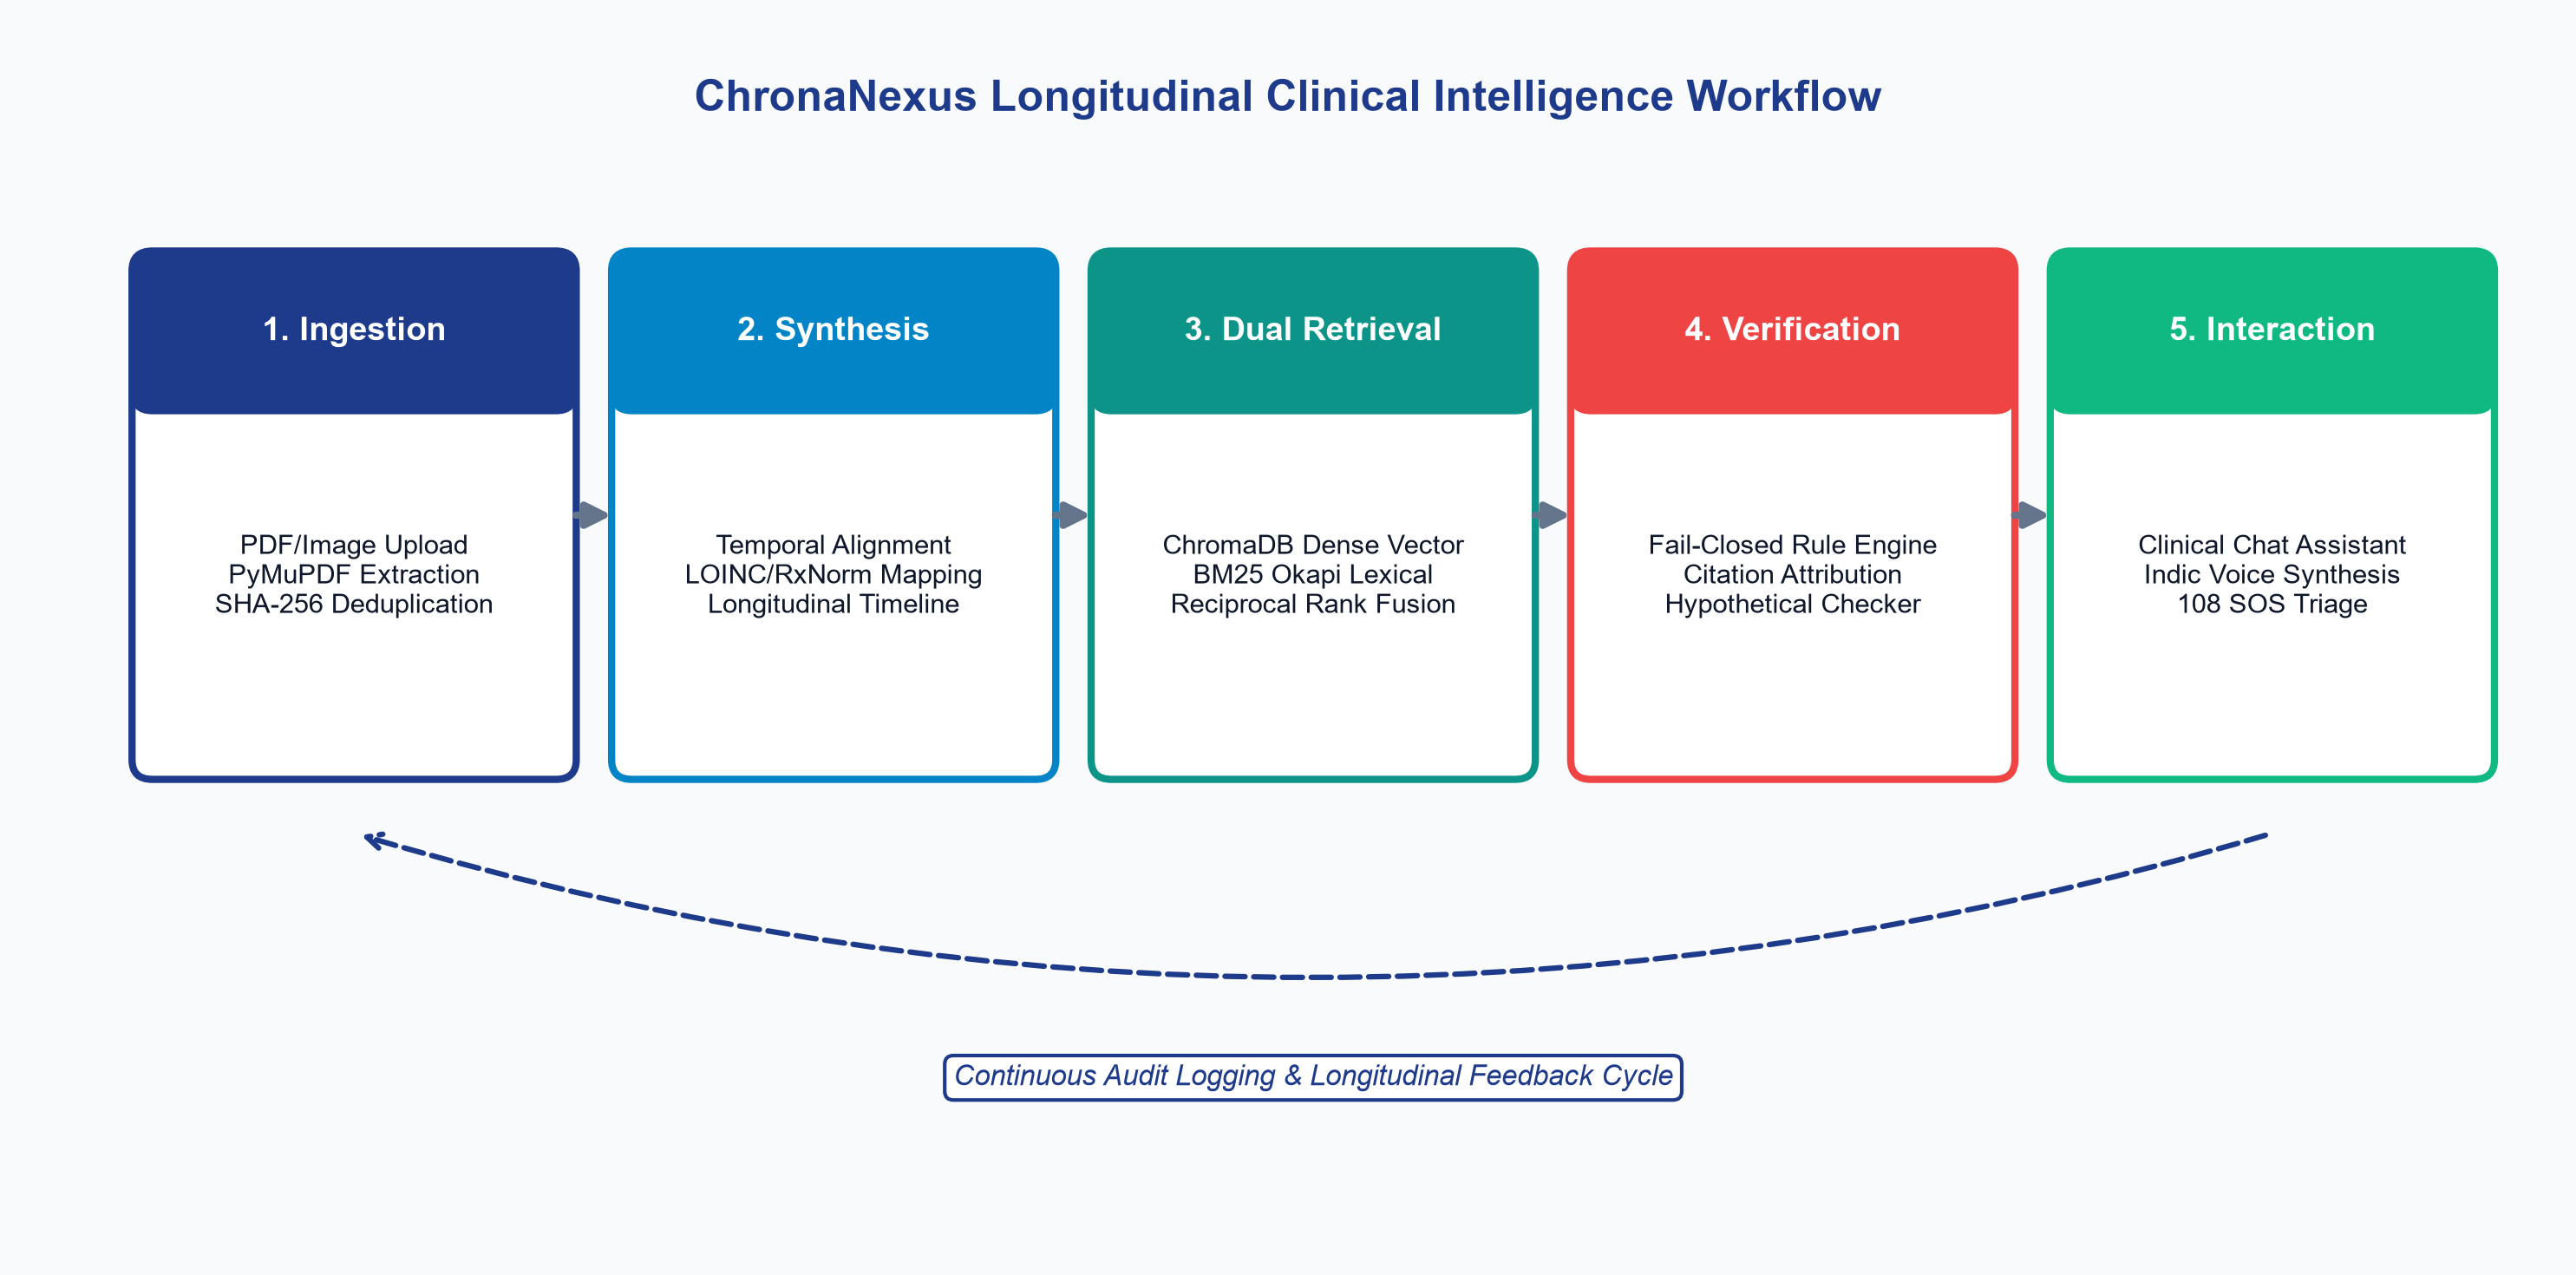
\includegraphics[width=0.96\linewidth]{figures/fig1_1_workflow.png}
    \caption{Conceptual workflow of the ChronaNexus clinical intelligence and verification lifecycle.}
    \label{fig:1_1_workflow}
\end{figure}

The workflow progresses through five systematic stages:
\begin{enumerate}
    \item \textbf{Ingestion and Deduplication}: Uploaded clinical documents undergo SHA-256 cryptographic hashing to eliminate redundant storage. \texttt{PyMuPDF} extracts raw textual strings and tabular bounding boxes, preserving spatial layout integrity.
    \item \textbf{Synthesis and Standardization}: Unstructured texts are parsed by regex-driven entity extractors mapped against standard medical ontologies (LOINC for laboratory tests, RxNorm for pharmaceutical formulations). Lab results are ingested into an ACID-compliant relational schema (\texttt{SQLite}) to enable instantaneous SQL mathematical aggregation.
    \item \textbf{Dual-Channel Retrieval}: Incoming clinical inquiries are split into two parallel query paths: dense vector semantic search against a local \texttt{ChromaDB} vector database (embedding $384$-dimensional vectors via \texttt{bge-small-en-v1.5}) and lexical inverted index search via BM25 Okapi. Reciprocal Rank Fusion merges both candidate sets into an optimal top-5 context window.
    \item \textbf{Hybrid Verification}: Generated responses from the language model are parsed into individual atomic claims. Tier 1 deterministic rules intercept numerical values, temporal bounds, and medication dosages, matching them against source chunks. Unresolved claims pass to Tier 2 neural natural language inference. If a claim fails verification, the engine fails closed, retracting the assertion or emitting a cautionary flag.
    \item \textbf{Multimodal Interaction and Dispatch}: Grounded clinical answers are delivered via an interactive web interface with verified citation badges, streamed via low-latency neural text-to-speech across six languages, or compiled into a compact JSON triage payload for emergency 108 dispatch.
\end{enumerate}


\section{Key Contributions of the Project}
\label{sec:intro_contributions}

The primary scientific, engineering, and architectural contributions of this work include:
\begin{enumerate}
    \item \textbf{Asymmetric Hybrid Symbolic-Neural Claim Verification}: Engineering a fail-closed verification pipeline that bridges the speed of deterministic symbolic rules ($<5\text{ ms}$) with the semantic reasoning of neural NLI, achieving $86.00\%$ verification accuracy and $100\%$ citation attribution precision on evaluated benchmark cases.
    \item \textbf{Empirical Analysis of Benchmark Leakage}: Discovering and documenting that trivial 5-rule regex heuristics achieve $100\%$ apparent verification on popular synthetic clinical benchmarks without consulting patient context, demonstrating the critical necessity of hybrid reasoning over naive prompt evaluations.
    \item \textbf{Privacy-First Local SLM Inference}: Implementing a fully functional on-device inference architecture utilizing local SLMs (via Ollama CPU inference) alongside cloud fallback (Groq Cloud LLM), achieving a mean query latency of $1.28\text{ s}$ (cloud) and $2.45\text{ s}$ (local) with zero unencrypted PHI leakage.
    \item \textbf{Unicode Phonetic Bridge for Indic Speech Synthesis}: Designing an offset mapping algorithm ($\Delta = -0x0180$) that translates Odia Unicode codepoints to isomorphic Bengali phonemes, unlocking high-cadence natural neural voice synthesis with zero accent distortion.
    \item \textbf{Comprehensive Automated Test Suite}: Engineering a suite of $190$ automated backend unit and integration tests distributed across $12$ pytest suites, featuring an active database interceptor that guarantees zero test pollution against persistent databases.
\end{enumerate}


\section{Organization of the Report}
\label{sec:intro_organization}

The remainder of this report is organized as follows:
\begin{itemize}
    \item \textbf{Chapter 2 (Literature Survey)}: Reviews foundational literature across clinical NLP, Retrieval-Augmented Generation, claim verification, and Indic speech synthesis, benchmarking academic and commercial systems.
    \item \textbf{Chapter 3 (System Analysis)}: Details the requirement analysis, stakeholder use cases (including UML Use Case diagrams), functional and non-functional specifications, and the comprehensive Requirements Traceability Matrix (RTM).
    \item \textbf{Chapter 4 (System Architecture and Design)}: Presents the 3-Tier system architecture, Data Flow Diagrams (DFD Level-0 and Level-1), UML sequence diagrams for authentication and clinical query flows, and the complete relational Entity-Relationship Diagram (ERD).
    \item \textbf{Chapter 5 (System Implementation)}: Documents the software engineering realization across six core backend subsystems and two delivery services, detailing Algorithms 5.1 through 5.4, database schema migration, and API route controllers.
    \item \textbf{Chapter 6 (Machine Learning and Data Pipeline)}: Explores the embedding representations, BM25 lexical tokenization, Reciprocal Rank Fusion, the 2-tier claim verification engine, and the Indic phonetic transliteration bridge.
    \item \textbf{Chapter 7 (Testing and Validation)}: Details the automated testing strategy spanning $190$ unit and integration tests across $12$ pytest suites, execution logs, and end-to-end verification test cases TC-01 through TC-20.
    \item \textbf{Chapter 8 (Cost and Sizing Analysis)}: Evaluates the computational resource sizing, memory footprint, hosting cost model, and open-source infrastructure savings.
    \item \textbf{Chapter 9 (Results and Discussion)}: Discusses quantitative retrieval performance, claim verification benchmark results, latency distributions, and an analysis of benchmark leakage.
    \item \textbf{Chapter 10 (Conclusion and Future Work)}: Summarizes the project deliverables, evaluates limitations, and charts future research directions towards direct HL7/FHIR interoperability and on-device quantization.
    \item \textbf{Chapter 11 (Appendix)}: Contains supplementary API requests, core source code listings, capstone development timeline, and clinical terminology catalogs.
\end{itemize}

\newpage
